\documentclass{beamer}

\usepackage{amsfonts}
\usepackage{amsmath}
\usepackage{longtable}
\usepackage{csquotes}
\usepackage{standalone}

\usepackage{graphicx}
\graphicspath{{../pictures/}}

\usepackage{tikz}
\usetikzlibrary{shapes, calc, arrows, decorations.markings,
  decorations.pathmorphing, decorations, patterns, chains, snakes,
  backgrounds, positioning, fit, petri}
\newcommand{\inputpicture}[1]{\input{../drawings/#1}}

\usepackage{listings}
\lstset{language=C, basicstyle=\ttfamily, breaklines=true, keepspaces=true,
  keywordstyle=\color{blue}}

\usepackage{bytefield}

\usefonttheme{professionalfonts}
\usefonttheme{serif}
\usepackage{fontspec}
\setromanfont{CMU Serif}
\setsansfont{CMU Sans Serif}
\setmonofont{CMU Typewriter Text}

\usepackage{hyperref}
\hypersetup{colorlinks=true, linkcolor=black, filecolor=black, citecolor=black,
  urlcolor=blue , pdfauthor=Evgenii Iuliugin <yulyugin@gmail.com>,
  pdftitle=Fundamentals of Full-Platform Simulation}

\usepackage{underscore}
\usepackage{amsthm}

\subtitle{Fundamentals of Full-Platform Simulation}
\subject{Lecture}
\date{\today}

\author[Evgenii Iuliugin]{
  Evgenii Iuliugin \small{\href{mailto:yulyugin@gmail.com}{yulyugin@gmail.com}}}
\typeout{Copyright 2021 Evgenii Iuliugin}

\usetheme{Berlin}
\setbeamertemplate{navigation symbols}{}

\newcommand{\finalslide}{
    {\huge{Thank you!}\par}

    \vfill
    Slides and material are available at
    \url{https://github.com/yulyugin/sim-lectures}
    \vfill

    \tiny{\textit{Note}: All trademarks are the property of their respective
        owners.
        The presented point of view reflects the personal opinion of the author.

        %All the materials are licensed under the Creative Commons
        %Attribution-NonCommercial-ShareAlike 4.0 Worldwide. To view a copy of
        %this license, visit
        %\url{http://creativecommons.org/licenses/by-nc-sa/4.0/}.
    }
}


\title{Simulation Through Interpretation}

\begin{document}

\startslides

\begin{frame}{On the Previous Lecture:}
Requirements for simulation:
\begin{itemize}
\item Accuracy,
\item Speed,
\item Compatibility.
\end{itemize}
\end{frame}

\begin{frame}{Questions}
\begin{itemize}
\item What units are used to measure simulation speed?\pause
\item How much slower is a cycle-accurate simulator than a functional?
\end{itemize}
\end{frame}

\begin{frame}{Simulated System}
\centering
\vfill
\inputpicture{cpu-mem}
\vfill
\end{frame}

\section{Pipeline}

\begin{frame}{Basic 5-Stage Pipeline}
\centering
\inputpicture{interpreter-cycle}
\end{frame}

\begin{frame}[fragile]{Switched interpreter}
\begin{lstlisting}
while (run) {
    raw_code = fetch(PC);
    (opcode, operands) = decode(raw_code);
    switch (opcode) {

    case opcode1:
        func1(operands); PC++; break;

    case opcode2:
        func2(operands); PC++; break;

    /*...*/
    }
}
\end{lstlisting}
\end{frame}

\section{Fetch}

\begin{frame}[fragile]{Fetch}
\texttt{data = mem[pc];}\pause
\vfill
Do not forget about address translation:
\begin{lstlisting}
paddr = v2p(pc); // pc is a virtual address
data = mem[paddr];
\end{lstlisting}
\end{frame}

% TODO: Add a slide about paging. People don't know about it at the moment.

\begin{frame}{Fetch}
<<Simple>> memory read?
\pause\bigskip
\begin{itemize}
\item Non-execute page.
\pause\bigskip
\item Unaligned accesses cause effects on some architectures.
\pause\bigskip
\item Cross-page accesses. \\
The pages may have different access rights.
\end{itemize}
\end{frame}

\section{Decode}

\begin{frame}{Decode}
Decoding --- translation of instruction data from machine code to internal
(high-level) representation suitable for further analysis.
\end{frame}

\begin{frame}{Example 1: RISC-V}
\centering
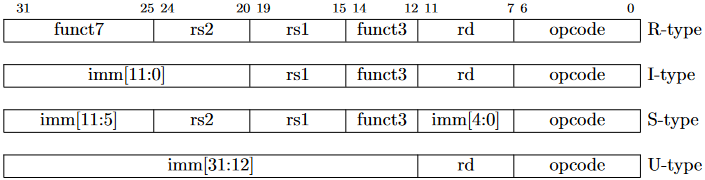
\includegraphics[width=.9\textwidth]{risc-v-formats}

\tiny{Source: The RISC-V Instruction Set Manual, Volume I: Unprivileged ISA,
      Document Version 20191213, page 16}
\end{frame}

\begin{frame}[fragile]{Example 1: RISC-V decoder (1/3)}
\begin{lstlisting}
#define BIT_FIELD(v, e, s) \
    (v >> s) & ((1 << (e - s + 1)) - 1)

static inline int32_t
sign_extend(uint32_t v, int width) {/* ... */};

typedef struct decode {
    uint32_t opcode;
    uint32_t rd;
    uint32_t rs1;
    uint32_t rs2;
    int32_t  imm;
    uint32_t funct3;
    uint32_t funct7;
} decode_t;
\end{lstlisting}
\end{frame}

\begin{frame}[fragile]{Example 1: RISC-V decoder (2/3)}
\begin{lstlisting}
decode_t
decode(uint32_t raw) {
    uint32_t op = BIT_FIELD(raw, 6, 0);
    switch (type(op)) {
    case I_type:
         return decode_i_type(raw);
    case R_type:
         return decode_r_type(raw);
    /../
    }
}
\end{lstlisting}
\end{frame}

\begin{frame}[fragile]{Example 1: RISC-V decoder (3/3)}
\begin{lstlisting}
decode_t
decode_i_type(uint32_t raw) {
    uint32_t op = BIT_FIELD(raw, 6, 0);
    uint32_t rd = BIT_FIELD(raw, 11, 7);
    uint32_t funct3 = BIT_FIELD(raw, 14, 12);
    uint32_t rs1 = BIT_FIELD(raw, 19, 15);
    int32_t imm = sign_extend(
        BIT_FIELD(raw, 31, 20), 12);

    return (decode_t){.op = op, .rd = rd,
                      .funct3 = funct3, .rs1 = rs1,
                      .imm = imm};
}
\end{lstlisting}
\end{frame}

\begin{frame}{Example 2: Intel\reg~IA-64}
\centering
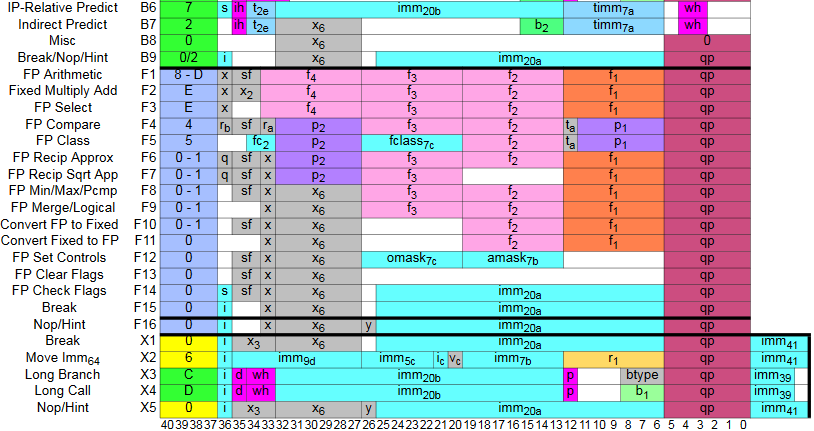
\includegraphics[width=.9\textwidth]{itanium-formats}

\tiny{Source: Intel\reg~Itanium\reg~Architecture Software
      Developer’s Manual, Revision 2.3, page 305}
\end{frame}

\begin{frame}{Example 3: Intel\reg~IA-32}
\centering
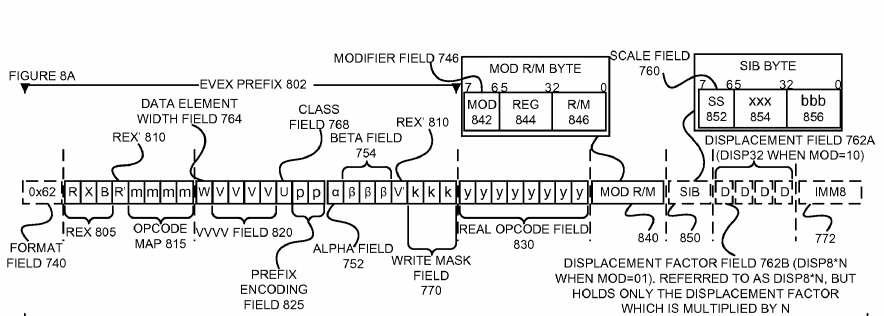
\includegraphics[width=.9\textwidth]{ia32-evex}

\tiny{J.C.S. Adrian et al. Systems, Apparatuses, and Methods for Blending Two
      Source Operands into a Single Destination Using a Writemask. US Patent
      Application Publication. \No~2012/0254588 A1}
\end{frame}

\begin{frame}{What to Fetch From Machine Code?}
\begin{centering}
\inputpicture{instruction-anatomy}
\end{centering}
\vfill
Input: machine code.

Output:
\begin{itemize}
\item Success, failure, not enough data.
\item In case of success: instruction length.
\item In case of success: information about operands.
\item In case of success: simulation routine.
\end{itemize}
\end{frame}

\begin{frame}{Decode}
\begin{itemize}
\item Decoders are usually generated from ISA description.
\item In general: classical problem of parser/synax analyser construction.
\item In practice: special tools and languages.
\item Example: Intel\reg~XED (x86 encoder-decoder). \url{https://github.com/intelxed/xed}
\end{itemize}
\end{frame}

\begin{frame}{Decode: harsh reality}
\begin{itemize}
\item Variable instruction lenght. Intel\reg~IA-32: from 1 to 15 bytes. How many bytes to decode at once?
\item Decoding results depends of prefixes and execution mode. Example: 0x40-0x4f in Intel\reg~IA-32/Intel\reg~64/AMD64.
\end{itemize}
\end{frame}

\begin{frame}{Disassemble}
\begin{itemize}
\item Disassemble --- translate from machine code into human readable
  representation (mnemonic, assembly).
\item Encode (assemble) --- translate from mnemonic to machine code.
\end{itemize}
\end{frame}

\section{Execute}

\begin{frame}{Execute}
\begin{itemize}
\item Basic block --- simulation function for one instruction (a.k.a.~service routine).
\item Service routines are tipically written in high-level programming
  languages: portable solution.
\item Generators are often used.
\item Example: SimGen --- single discription is used to generate decoder,
  disassembler and service routines.
\end{itemize}
\end{frame}

\begin{frame}[fragile]{Simulated state}
\begin{lstlisting}
typedef struct {
    uint32_t pc;

    uint32_t regs[16];

    bool z_flag;
    bool n_flag;
    bool o_flag;
    bool c_flag;
} cpu_t;
\end{lstlisting}
\end{frame}

\begin{frame}[fragile]{Example: ADD reg reg reg}
\begin{lstlisting}

void add32_rrr(cpu_t *cpu, int src1, int src2, int dst) {
    cpu->regs[dst] = cpu->regs[src1]
                   + cpu->regs[src2];
\end{lstlisting}
\pause

\begin{lstlisting}
    cpu->z_flag = cpu->regs[dst] == 0;
    cpu->n_flag = cpu->regs[dst] & (1 << 31);
    cpu->o_flag = cpu->regs[dst] < 
            MAX(cpu->regs[src1], cpu->regs[src2]);
    cpu->c_flag = calc_c_flag(cpu->regs[src1],
                              cpu->regs[src2]);
}
\end{lstlisting}
\end{frame}

\begin{frame}{Intel\reg~IA-32 CALL}
\centering
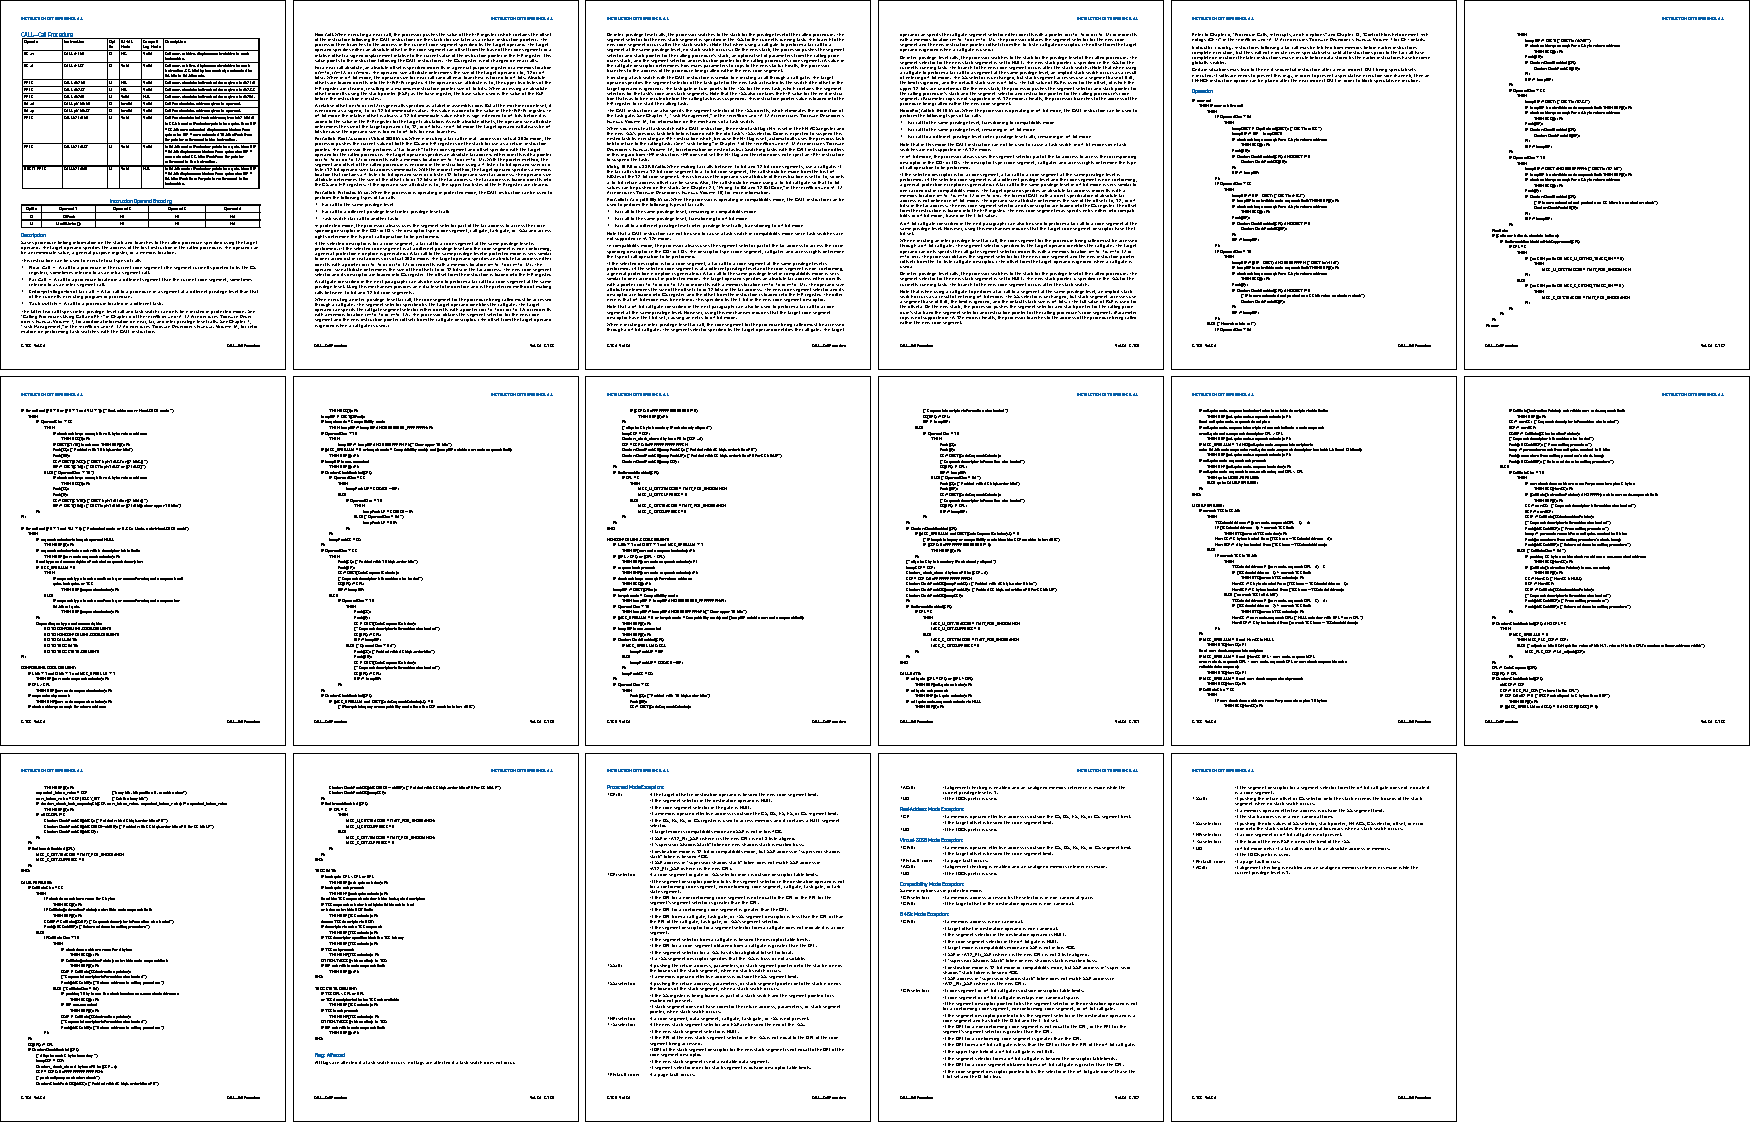
\includegraphics[width=\textwidth]{ia32-call}

\tiny{Source: Intel\reg~64 and IA-32 Architectures Software Developer’s Manual,
      Order Number: 325462-073US, pages 716-732.}
\end{frame}

\section{Memory}

\begin{frame}[fragile]{Memory}
<<Ordinary>> memory access:
\vfill
\begin{lstlisting}
write_mem(cpu, dst_addr, data, size);
data = read_mem(cpu, dst_addr, size);
\end{lstlisting}
\pause\vfill
\begin{itemize}
\item Attempt to change read-only memory,
\item Unaligned address,
\item Cross-page access.
\end{itemize}
\end{frame}

\section{Exceptions}

\begin{frame}{Accurate Pipeline}
\centering
\resizebox{9cm}{7cm}{\inputpicture{interpreter-cycle-exception}}
\end{frame}

\begin{frame}{Classification}
\begin{itemize}
\item Exception --- synchronous, without repeating of current instruction.
\item Fault --- synchronous, with repeating of current instruction.
\item Trap --- synchronous, without repeating of current instruction, intentoinal.
\item Interrupt --- external, asynchronous.
\item Abort --- external, asynchronous, no return point.
\end{itemize}
\end{frame}

\section{Write-Back}

\begin{frame}{Write-Back}
\begin{itemize}
  \item Processor state should be updated after all excecption checks to avoid
    partially changed state.
  \bigskip
  \item Advance \texttt{\$PC}:
  \pause\bigskip
  \begin{itemize}
    \item For most instructions: \texttt{\$PC += instruction_length}. \\
    Exception: \texttt{REP MOVS}.
    \pause\bigskip
    \item Explicit \texttt{\$PC} update --- control-flow instructions:
    \begin{itemize}
      \item (Un)conditional (In)direct Jump/Branch,
      \item Call/Return (subroutine).
      \item System call/return.
      \item ...
    \end{itemize}
  \end{itemize}
\end{itemize}
\end{frame}

\section{Improved Interpretation}

\begin{frame}{Pros and Cons}
\begin{itemize}
\item Implemented in high-level language --- portable.
\item Simple structure: reliable, extensible, re-usasble.
\pause
\item (Extremely) low simulation speed.
\end{itemize}
\end{frame}

\begin{frame}[fragile]{Where Is the Time Spent?}
\begin{lstlisting}
start: interruption = false;
while (!interruption) {
    raw_code = fetch(PC);
    (opcode, operands) = decode(raw_code); // <-- here
    switch (opcode) { // <-- and here
    case opcode1:
        func1(operands); PC++; break;
    case opcode2:
        func2(operands); PC++; break;
    /*...*/
    }
}
handle_interruption();
goto start;
\end{lstlisting}
\end{frame}

\begin{frame}[fragile]{Threaded Interpretation}
Jump right to the next instruction instead of start of the loop:
\bigskip
\begin{lstlisting}
func0: /* simulate instr0 */; PC++;
  next_opcode = decode(fetch(PC));
  goto func_ptr[next_opcode];
func1: /* simulate instr1 */; PC++;
  next_opcode = decode(fetch(PC));
  goto func_ptr[next_opcode];
func2: /* simulate instr2 */; PC++;
  next_opcode = decode(fetch(PC));
  goto func_ptr[next_opcode];
\end{lstlisting}

\tiny\url{http://stackoverflow.com/questions/11227809/why-is-processing-a-sorted-array-faster-than-an-unsorted-array}
\end{frame}

\begin{frame}{Cached Interpretation}
\begin{itemize}
\item Usually guest code is static.
\item It's highly probable that an instruction with some \texttt{\$PC} will be
  executed many times.
\item Why decode every time?
\item Solution: create a cache mapping instruction address to decode data.
\end{itemize}
\end{frame}

\begin{frame}[fragile]{Cached Interpretation}
\begin{lstlisting}
while (!interruption) {
  if (operation = cache[PC]); // shortcut
  else { // not cached, full path
    operation = decode(fetch(PC));
    cache[PC] = operation; // cache the result
  }
  switch (operation) {
     /* ... */
  }
}
\end{lstlisting}
\end{frame}

% TODO: slide with diagram.

\begin{frame}{Cached Interpretation}
\begin{itemize}
\item Cache size is limited.
\item Old data needs to be removed from the cache.
\item Code modifications need to be tracked. Otherwise cache will have invalid
  data.
\end{itemize}
\end{frame}

\section{Conclusions}

\begin{frame}{Conclusions}
\begin{itemize}
\item Basic 5-stage pipeline.
\item Decoder, disassembler, encoder.
\item Switched interpreter.
\item Threaded interpreter.
\item Cached interpreter.
\item Exeption, Interrupt, Trap, Fault\dots
\end{itemize}
\end{frame}

\begin{frame}[allowframebreaks]{Bibliography}
\begin{thebibliography}{99}
  \bibitem{} \textit{D. Mihoka, S. Shwartsman}. Virtualization Without Direct
    Execution or Jitting: Designing a Portable Virtual Machine Infrastructure.
  \bibitem{} \textit{Y. Lifshitz, R. Cohn, I. Livni, O. Tabach, M. Charney, K.
    Hazelwood}. Zsim: A Fast Architectural Simulator for ISA Design-Space
    Exploration.
  \bibitem{} \textit{F. Larsson, P. Magnusson, B. Werner}. SimGen: Development of
    Efficient Instruction Set Simulators.
  \bibitem{} \textit{A. Sepp, J. Kranz, A. Simon}. GDSL: A Generic Decoder
    Specification Language for Interpreting Machine Language.
\end{thebibliography}
\end{frame}

\begin{frame}{On the Next Lecture:}
\begin{itemize}
\item Just In Time Compilation:
\begin{itemize}
\item Template-Based Translation,
\item Interpmediate Representation,
\item Problems.
\end{itemize}
\end{itemize}
\end{frame}

\finalslide

\end{document}
